\documentclass[10pt]{article}
\usepackage[polish]{babel}
\usepackage[utf8]{inputenc}
\usepackage[T1]{fontenc}
\usepackage{amsmath}
\usepackage{amsfonts}
\usepackage{amssymb}
\usepackage[version=4]{mhchem}
\usepackage{stmaryrd}
\usepackage{graphicx}
\usepackage[export]{adjustbox}
\graphicspath{ {./images/} }

\begin{document}
\begin{enumerate}
  \item Punkty \(D\) i \(E\) leżą odpowiednio na bokach \(B C\) i \(A B\) trójkąta równobocznego \(A B C\), przy czym \(B E=C D\). Punkt \(M\) jest środkiem odcinka \(D E\). Wykazać, że
\end{enumerate}

\[
B M=\frac{1}{2} A D
\]

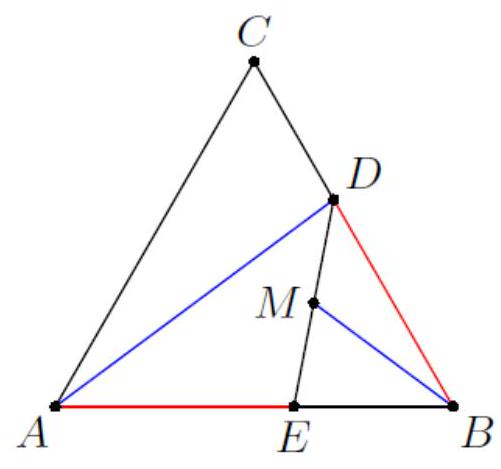
\includegraphics[max width=\textwidth, center]{2024_11_21_b24afab5947f4ac78933g-1}\\
2. Udowodnij, że jeżeli trójkąt ma dwie środkowe jednakowej długości, to jest równoramienny.\\
3. Rozwiąż równanie

\[
\sqrt{x-2 \sqrt{x-1}}+\sqrt{x+2 \sqrt{x-1}}=\frac{1}{x-1}
\]


\end{document}